In \cite{Paper3} the authors used the new H.265 codec (unlike in the other two papers) for their approach. In their work they present a CPU plus GPU parallel encoding framework which targets the critical bottlenecks like Variable Block Size Motion Estimation (VBSME) of the encoding algorithm and optimises the data flow between the two devices. The proposed framework is shown in figure \ref{hevc_framework}

\begin{figure*}[ht]
\centerline{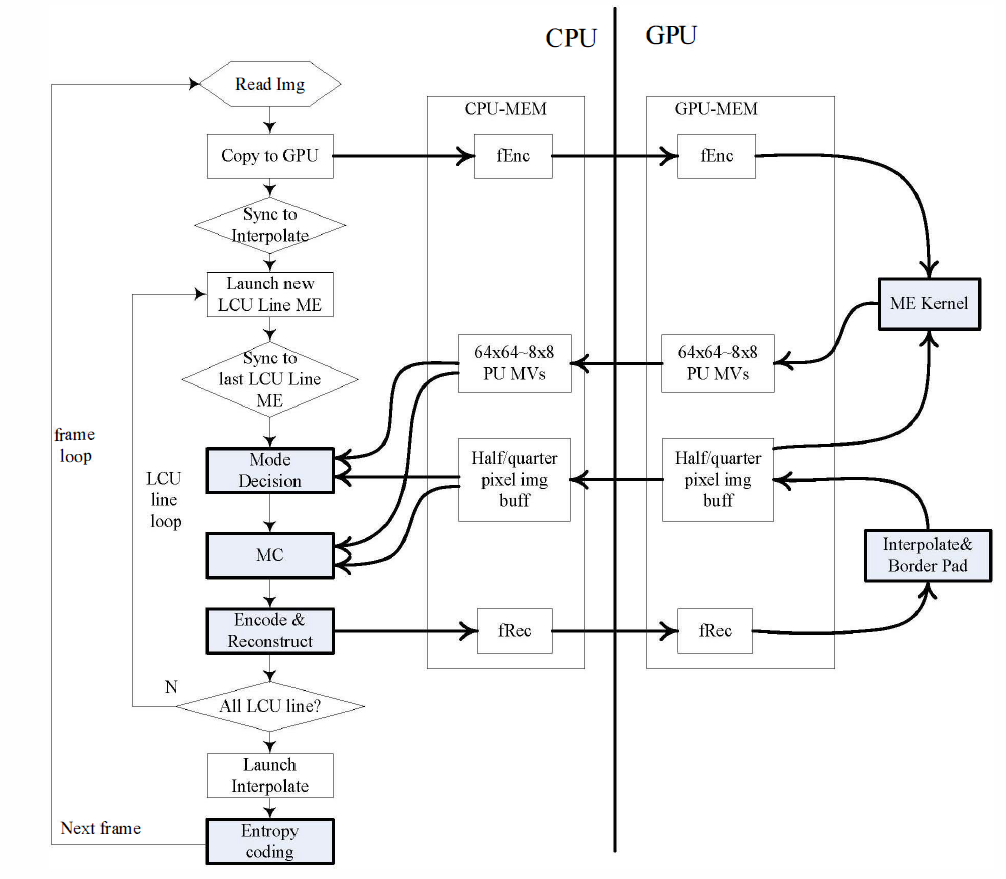
\includegraphics[scale=0.5]{pics/hevc_framework}} % The bounding box is set manually in this example. Useful for some .pdf figures.
\caption{\label{hevc_framework}{\it Parallel encoding framework on CPU plus GPU platform.
The thick lines with arrows represent the dataflow directions. (taken from \cite{Paper3})}}
\end{figure*}

The authors divided the HEVC encoder for their framework into six components: VBSME, mode decision, motion compensation, interpolation, encode plus reconstruction and
entropy coding. The VBSME and Interpolation components,
the right part in figure \ref{hevc_framework}, run on GPU, the others run on
CPU. \\
The ME is like mentioned before very compute intensive and therefore executed on the GPU. In comparison to the other papers the framework considers the MVs dependencies during the ME process. \\
Interpolation is also run on the GPU since it has a fast interpolation unit. The other tasks like mode decision, motion compensation, encode, reconstruct and entropy coding are all run on a CPU.\\
To successfully run the different parts of the algorithm in parallel on both CPU and GPU two synchronisation components are used: 'Sync to Interpolate' and 'Sync to last CTU Line ME'. They ensure that both devices wait for each other if necessary.\\
The mode decision process is according to the authors the bottleneck of this framework and therefore they decided to implement a fast prediction unit partition scheme. This scheme has a maximum of 6 steps and chooses the mode for motion compensation in a faster way than the standard mode decision of the HM encoder \cite{hmencoder}. Of course the speed increase in 
mode decision indicates a possible loss in quality due to some mode decisions that would not be the best.
